\documentclass{tise_style_doi}

\usepackage{soul}     % for highlighting
\usepackage{upquote}  % for correct display of single quotes in verbatim
\usepackage{booktabs} % for toprule, etc. in tabular
\usepackage{pifont}   % used to create check/x marks

\newcommand{\cmark}{\ding{51}} % check mark
\newcommand{\xmark}{\ding{55}} % x mark

%--------------------------------------------------------------------------------
%<--- TYPE WITHIN THESE BOUNDS  ------------------  TYPE WITHIN THESE BOUNDS --->
%12345678901234567890123456789012345678901234567890123456789012345678901234567890
%--------------------------------------------------------------------------------

\title{DataCamp: An Interactive Learning Tool for Programming}

\begin{document}

\maketitle

%================================================================================
\section{Introduction}

%\doublespacing

It is no surprise that technology plays a vital role in the field of statistics. As
the technological revolution continues to unfold, the use of statistical software
has become increasingly emphasized in education \citep{AmericanStatisticalAssociation2016}.
By integrating the capabilities of technology in statistics courses, students can
explore fundamental concepts by analyzing and interpreting real data sets
\citep{Chance2007, Hardin2015, Horton2014}, giving them an authentic view of how statistics
is practiced outside of the classroom \citep{Wang2017}.

As the stated goal of a statistics course is to help students develop the ability to think
statistically \citep{AmericanStatisticalAssociation2016}, introducing technology into
the curriculum can greatly strengthen this ability by illustrating concepts such as
variability, randomness and hypothesis testing. Although numerous statistical technologies
exist, R and RStudio provide extensive computational abilities (free of charge) and are
commonly used in statistics courses. R allows students to explore real-world data sets which
can not only enhance their understanding of concepts, but can also spark an interest in the
domain of statistics \citep{Wang2017}.

\hl{Discuss benefits of `learn by doing' or repetition?  Ie, this incorporates
more student practice with typing code.}

%--------------------------------------------------------------------------------
\subsection{Interactive tools to learn R}

With the increased use of R in classrooms, an effective tool to familiarize students
with statistical software is needed \citep{Baumer2014}. While R software provides users
with extraordinary statistical capabilities, there is certainly a steep learning curve.
To facilitate this transition to R programming, popular interactive teaching technologies
have been created including Try R, \texttt{swirl}, \texttt{learnr}, and DataCamp.
Interactive tools allow students to actively work through coding problems and receive
immediate feedback.  See Table \ref{tab:compare} for a comparison of existing
technologies.

\hl{Best placement for this table?}

\begin{table}
\begin{tabular}{lcccc}
\toprule
Feature                      & Try R  & \texttt{swirl}    & \texttt{learnr} & DataCamp \\
\midrule
%Requires R installation     & \cmark & \cmark            &  $\sim$         & \xmark   \\
Web-based                    & \cmark & \xmark            &  $\sim$         & \cmark   \\
Tracks student progress      & \xmark & $\sim$            &  \xmark         & \cmark   \\
Integrates with LMS          & \xmark & \xmark            &  \xmark         & \cmark   \\
Variety of lessons available & \xmark & \cmark            &  \xmark         & \cmark   \\
Educators can create content & \xmark & \cmark            &  \cmark         & \cmark   \\
%Meta-data available         & \xmark &   ?               &                 & \cmark   \\
\bottomrule
\end{tabular}
\caption{Comparison of interactive technologies to learn programming in R.
For web-based applications, R installation is not required.}
\label{tab:compare}
\end{table}

%--------------------------------------------------------------------------------
\subsubsection{Try R}

Try R is web-based interactive R programming course that consists only of
codding exercises \citep{TryR}. The RStudio console
can be intimidating to new statistics students
so an  advantage of a web-based teaching tool is the clean and easy to use interface.
User-friendliness is an important quality given that students often struggle more
with the software used than the statistical concepts themselves \citep{Hare2017}.
When students only need their web browser to participate, all installation
complications are avoided and valuable class time can be focused on the lesson.
However, Try R is not open source so public content authoring is not available;
educators are limited to the existing lessons available on the Try R website.
Lastly, Try R does not currently integrate with learning management systems (LMS).

%--------------------------------------------------------------------------------
\subsubsection{swirl}

\texttt{swirl} is an open source R package where students can learn R programming
directly in the R console (so it requires a local R installation) \citep{Kross}.
This interactive learning tool incorporates both code exercises and multiple choice
questions. \texttt{swirl} contains several pre-existing lessons, and
educators can also create their own lesson content to fit
specific curriculum \citep{Carchedi2014}.  While \texttt{swirl} can be linked to Massive
Open Online Courses (MOOCs) like Coursera, integration of LMS
is not currently available.

%--------------------------------------------------------------------------------
\subsubsection{learnr}

\texttt{learnr} is an open source R package that converts R Markdown documents
to programming tutorials using Shiny \citep{GarrettGrolemund2017}.  These
tutorials can consist of code exercises, multiple choice questions, videos,
and interactive Shiny components.  \texttt{learnr} enables instructors to
write their own programming tutorials, but there is not a collection of readily available
lessons.  Although the ``hint'' options in \texttt{learnr}
are minimal, the \texttt{checkr} package works with \texttt{learnr} to provide
tailored feedback \citep{DanielKaplan2018}.  \texttt{learnr} tutorials can be deployed either
locally on a user's computer (requires R installation) or through a Shiny Server (web-based).
This interactive tutorial does not allow for tracking of student progress.



%================================================================================
\section{Introduction to DataCamp}

\hl{Weston - insert background here}
DataCamp (\url{www.datacamp.com}) was first created in 2013 with the mission to 
``democratize data science education world wide''.
DataCamp provides a comprehensive web-based platform to interactive lessons on various coding
languages. The DataCamp website offers free `community' courses
as well as more specialized \textit{Premium} classes that require a fee. However, when used
for academic purposes the \textit{Premium} DataCamp content is free for up to six months.
Currently, DataCamp has 2.5 million users across virtually all countries.

%--------------------------------------------------------------------------------
\subsection{Accessibility}

DataCamp lessons are available through the both the DataCamp website and a mobile app
(\url{https://www.datacamp.com/mobile}) so students can access lessons through their
web-browser on a laptop, tablet or mobile device.  This makes learning programming
accessible to anyone with an internet connection and negates the barrier of software installation.

%--------------------------------------------------------------------------------
\subsection{Courses}

There are currently 114 premium courses created by 82 instructors, and this
number is constantly growing.  Courses span a wide range of languages (R, Python, SQL,
Git, and shell) as well as topics (programming, data manipulation, data visualization,
statistical methods, etc.).  The breadth of courses offered makes DataCamp suitable
for novice students to advance programmers. If there is not a course that quite
fits your needs, you can also create your own community course (see Section \ref{creating}).

%--------------------------------------------------------------------------------
\subsection{Modularity}

DataCamp courses are broken up into chapters and each chapter is composed of modular
exercises. Modularity is a critical component in designing a learning tool because it
allows independent pieces to be added, modified or removed from the entire functionality
\citep{Hare2017}. This is particularly useful when creating your own course as DataCamp
course exercises can be added, modified, or deleted as new topics arise and instructors
can tailor these exercises to meet the needs of a particular class.

%--------------------------------------------------------------------------------
\subsection{Gamification}

Each exercise is given a specified number of redeemable points which the students
can see when they begin the exercise, introducing a gamification feature to the learning
experience. When in a classroom group, students can view their progress (points and chapters
completed) \hl{as well as the progress of their peers - verify}. Furthermore, when students
can see the number of available points for an exercise it can motivate them to meet their personal
achievement goals \citep{Chang2016}. If the student completes an exercise without
any assistance, they will receive the full points. If the student is having difficulty, they can
view the exercise `hint' option and 30 percent of the available points are deducted.
Lastly, if the student is completely stuck the student may view the solution; however, all
points are deducted.

%--------------------------------------------------------------------------------
\subsection{Tracking student progress}

A notable feature that sets DataCamp apart from competing technologies is the ability
to track student progress. This means that programming courses can be used
in the classroom in a number of ways: as traditional homework assignments, as an activity
during lab periods, as pre-class assignments for a flipped classroom, and even as a
test or assessment tool.

In order to utilize DataCamp's \textit{classroom} benefits, first create an academic
group on the website \url{https://www.datacamp.com/groups/education}. After your
university information has been verified and the classroom account has been approved,
access is facilitated by either creating a group through the DataCamp website or
linking directly to your LMS.

If using the group functionality on the DataCamp website, you can add students to the course
by their university email address on the \textit{Members} tab.  You can also set deadlines
for assignments (entire courses or individual chapters) and view downloadable grade reports.

Alternatively, students can be linked to DataCamp assignments via an LMS (including
Blackboard, Moodle, Sakai, Canvas, EdX, Coursera, and Schoology) in the \textit{Settings} tab.
With direct LMS integration educators do not have to add students via their email address.
Furthermore, they can link directly to specific assignments in their LMS, and grades are
automatically recorded in the LMS grade book.

%================================================================================
\section{Creating a DataCamp course}
\label{creating}

%--------------------------------------------------------------------------------
%\subsection{Getting Started}

To build a course on DataCamp you need both a DataCamp account and a GitHub account
(\url{https://github.com}). Once logged into DataCamp as user, it is hard to find a link
to the \emph{teach} site - just go to \url{www.datacamp.com/teach/}.
Every DataCamp course is linked through GitHub version control, allowing educators to
easily collaborate and maintain code. While comprehensive documentation is provided
through the \emph{teach} website, we will discuss the basics.

The simplest way to begin building the course is to use the template course files from
the \textit{Create Course} dialog. This will automatically create a GitHub repository
that is linked to DataCamp.

%--------------------------------------------------------------------------------
\subsection{Initial repository}

The newly created GitHub repository will contain three files:
\begin{enumerate}
\item \texttt{README.md}
\item[] Contains helpful information on how to get started and cites resources to
learn more about the process.
\item \texttt{course.yml}
\item[] Contains general information about the course you are creating: title, university,
description, difficulty level, etc.
\item \texttt{chapter1.Rmd}
\item[] A template chapter file with examples of `normal' iterative coding exercises and
multiple choice questions.  To add more chapters to an R course, create new files in the repository
and name them \texttt{chapter1.Rmd}, \texttt{chapter2.Rmd}, \texttt{chapter3.Rmd}, etc.
\end{enumerate}

%--------------------------------------------------------------------------------
\subsection{Course editing}

Course creators can edit their courses through either GitHub or the \textit{Teach Editor}
accessed through the DataCamp website. The \textit{Teach Editor} allows content
creators to edit, preview, save changes, and synchronize to the GitHub repository.
Editing completed via GitHub does not allow for automatic content viewing. Any changes
that are made through the DataCamp \textit{Teach Editor} will update the GitHub
repository and vice versa.

%--------------------------------------------------------------------------------
\subsection{Components of a DataCamp lesson}

DataCamp lessons can consist of coding exercises, multiple choice exercises,
and videos.  Each exercise is presented as a multi-panel layout that consists
of an exercise body, instructions, script editor, and R console.  Exercises
can be initiated through creation buttons available in the \texttt{Teach Editor},
which automatically create an exercise template.

%~~~~~~~~~~~~~~~~~~~~~~~~~~~~~~~~~~~~~~~~~~~~~~~~~~~~~~~~~~~~~~~~~~~~~~~~~~~~~~~~
\subsubsection{Exercise layout}

Figure \ref{fig:code1} is an example of ``normal exercise'' syntax and Figure
\ref{fig:preview} is the corresponding student interface. Students read the
lesson information and instructions, answer the question, and submit their code.

\hl{It looks like the exercise header (yaml) has updated since last summer - update this?}

\hl{Take all examples from Intro to R course rather than personal course?}

\begin{figure}
\begin{Verbatim}[frame=single]
--- type:NormalExercise lang:r xp:100 skills:1 key:9a4fea2da0

## Visualizing quantitative data in R

We can visualize quantitative data with a *histogram*.

- use `hist(dataset$quant_var)` to create a histogram

*** =instructions
- Create a histogram of the `wage` variable from the `CPS85` data set
using the `hist()` function.
- Click the 'Submit Answer' Button and take a look at the R output in the
console.

*** =hint

*** =pre_exercise_code
```{r}
library(mosaicData)
```

*** =sample_code
```{r}
# Create histogram of wage variable with hist() function

```

*** =solution
```{r}
# Create histogram of wage variable with hist() function
hist(CPS85$wage)
```

*** =sct
```{r}
test_function("hist", args = "x",
              incorrect_msg = "Follow the format: `hist(dataset$variable)`
                               with specified dataset and variable.")
```

\end{Verbatim}
\caption{Syntax to create a ``normal exercise'' on DataCamp.  In DataCamp's
\texttt{Teach Editor}, the syntax is color-coded. \hl{Just include
screenshot here instead of verbatim so color coding is visible?}}
\label{fig:code1}
\end{figure}

\begin{figure}[h]
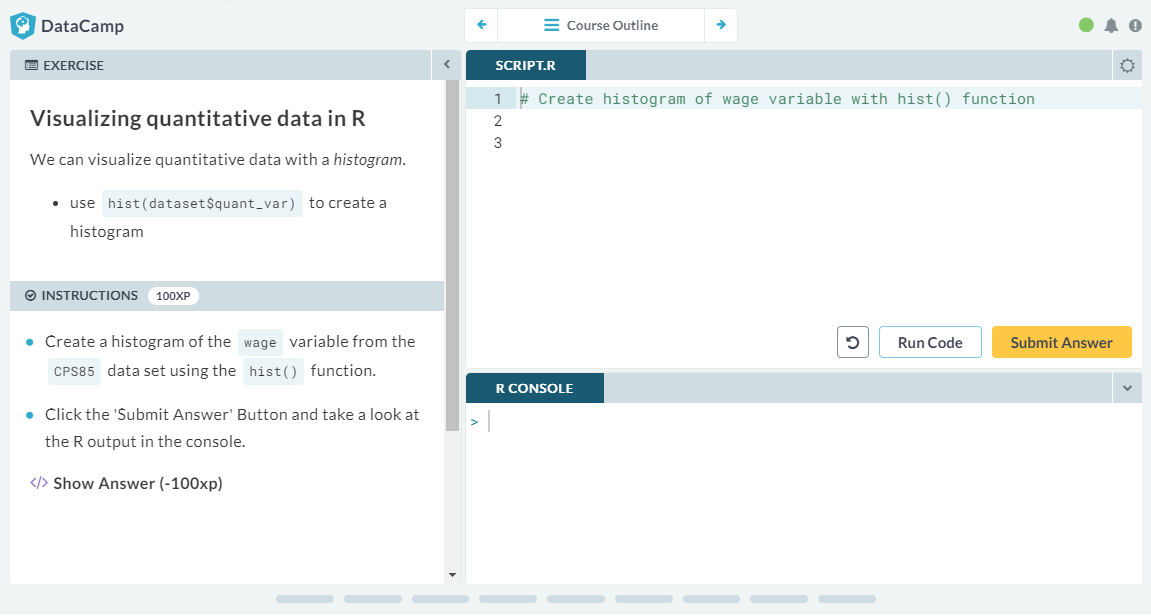
\includegraphics[width = 1.0\textwidth] {code1preview.png}
\caption{Preview of the rendered result of the ``normal exercise'' syntax displayed
in Figure \ref{fig:code1}.}
\label{fig:preview}
\end{figure}

%~~~~~~~~~~~~~~~~~~~~~~~~~~~~~~~~~~~~~~~~~~~~~~~~~~~~~~~~~~~~~~~~~~~~~~~~~~~~~~~~
\subsubsection{Exercise header}

When creating a new exercise, DataCamp automatically produces the header (the first line
of syntax). The header specifies the type of exercise (\texttt{type}), programming
language (\texttt{lang}), available points (\texttt{xp}), skills learned (\texttt{skills})
and a \texttt{key}. By default, DataCamp assigns 100 points to normal coding exercises,
but this value can be modified. The \texttt{skills} portion of the header refers to DataCamp's
eight different skill sets, defined by numbers 1-8. Skills and their corresponding
numbers can be found in the DataCamp documentation
\url{https://www.datacamp.com/teach/documentation#tab_gamification}.
Lastly, the \texttt{key} acts as a unique identifier for that exercise, allowing you
to modify content without losing any student data. In Figures \ref{fig:code1} and
\ref{fig:preview}, the \texttt{type} is Normal, the language is R,
the available points is 100xp and the skills learned is 1 (which corresponds to R Programming).

\hl{skills not used anymore? - link goes to a different page}

%~~~~~~~~~~~~~~~~~~~~~~~~~~~~~~~~~~~~~~~~~~~~~~~~~~~~~~~~~~~~~~~~~~~~~~~~~~~~~~~~
\subsubsection{Exercise body}

In the \textit{lesson} portion of the exercise (not labeled but below the header),
instructors can add additional information about the assignment that will help
students understand and complete the instructions. The \textit{instructions} section
contains the actual task required; instructors can also include
a \textit{hint} for extra guidance (optional). The \textit{pre-exercise code} sets up
the R work space for the student - here, you can automate tasks for the students such
as loading packages, importing data sets, or pre-processing data. The \textit{sample code}
section contains comments and code that will be visible to students in the R script
panel, which is where students submit code.  The correct answer to an exercise is
coded in the \textit{solution} section.  After student clicks the \texttt{Submit Code}
 button, their answer passes through the \textit{submission correctness test} (SCT)
where the submission is assessed for accuracy.

%~~~~~~~~~~~~~~~~~~~~~~~~~~~~~~~~~~~~~~~~~~~~~~~~~~~~~~~~~~~~~~~~~~~~~~~~~~~~~~~~
\subsubsection{Submission correctness test}

The SCT automatically assesses if the correct code was submitted \citep{Vankrunkelsven2016}.
If a student submits an incorrect answer, they will receive immediate feedback and guidance towards
the correct answer.  The SCT is executed through DataCamp's \texttt{testwhat} R
package (\url{https://github.com/datacamp/testwhat/wiki}). The \textit{testwhat} package
contains functions that test different types of problems including multiple choice
exercises, what students typed, and output generated.  The SCT compares the ideal answer
(from the solution code) to the student's answer. Various arguments can be added to the
test functions to adjust the testing process and feedback.  Instructors can either use the
default feedback that DataCamp automatically generates or write their own custom messages.
For example, Table \ref{tab:SCT} contains the default feedback for a few possible incorrect submissions
of the \texttt{hist()} function from the example
exercise \textit{Visualizing quantitative data in R} shown in Figures \ref{fig:code1} and
\ref{fig:preview}.

\hl{I don't think I have fully utilized the power of SCT in my example because
you can link multiple SCTs together, right?  Could use a different example.}

\begin{table}
\begin{tabular}{lll}
\toprule
Student submission & R console & SCT feedback \\
\midrule
\texttt{histogram(CPS85\$wage)} & Error: could not find & Have you called hist()? \\
                                & function ``histogram'' & \\
[2ex]
\texttt{hist(wage)} & Error: object `wage' & Follow the format: hist(dataset\$variable) \\
                    &  not found           & with specified dataset and variable.\\
[2ex]
\texttt{hist(CP85\$wage)} & Error: object `CP85' & Follow the format: hist(dataset\$variable) \\
                               & not found       & with specified dataset and variable. \\
[2ex]
\texttt{hist(CPS85\$wage)} & & Great work! \\
\bottomrule
\end{tabular}
\caption{Feedback provided in the R console and in the DataCamp lesson through the
SCT for the exercise shown in Figures \ref{fig:code1} and \ref{fig:preview}.}
\label{tab:SCT}
\end{table}

%--------------------------------------------------------------------------------
\subsection{DataCamp exercises}

DataCamp courses currently have six different exercise types available (see
Table \ref{tab:exercises}).

\begin{table}
\begin{tabular}{ll}
\toprule
Type & Description \\
\midrule
\texttt{VideoExercise}              & Displays a video exercise \\
\texttt{NormalExercise}	            & Instructions, exercise, code editor, and console \\
\texttt{MultipleChoiceExercise}     & Multiple choice question and console \\
\texttt{PureMultipleChoiceExercise} & Multiple choice question without a console \\
\texttt{TabExercise}	            & A series of connected sub-exercises \\
\texttt{BulletExercise}	            & A series of connected sub-exercises \\
\bottomrule
\end{tabular}
\caption{Exercise types currently supported in DataCamp}
\label{tab:exercises}
\end{table}

%~~~~~~~~~~~~~~~~~~~~~~~~~~~~~~~~~~~~~~~~~~~~~~~~~~~~~~~~~~~~~~~~~~~~~~~~~~~~~~~~
\subsubsection{Video exercise}

A \texttt{VideoExercise} displays as instructional video while relevant
slides appear in the background.

%~~~~~~~~~~~~~~~~~~~~~~~~~~~~~~~~~~~~~~~~~~~~~~~~~~~~~~~~~~~~~~~~~~~~~~~~~~~~~~~~
\subsubsection{Normal exercise}

A \texttt{NormalExercise} prompts students to submit code. The components of this
include: lesson section, instructions, pre-exercise code, sample code, hint, solution
and submission correctness testing code (SCT). The students interface consists of the
lesson, instructions, R script panel and R console (Figure \ref{fig:code1}).

%~~~~~~~~~~~~~~~~~~~~~~~~~~~~~~~~~~~~~~~~~~~~~~~~~~~~~~~~~~~~~~~~~~~~~~~~~~~~~~~~
\subsubsection{Multiple choice exercises}

The \texttt{MultipleChoiceExercise} contains a question and a list of various answers.
This exercise is accompanied by the R console and R output, and allows instructors to
pre-program objects or plots that the student needs to access to answer the question.
The \texttt{PureMultipleChoiceExercise} contains a question and a list of various
answers - this exercise type does not include the R console and output.
%Similar to a
%\texttt{NormalExercise}, the lesson, instructions, hint, pre-exercise code and SCTs are
%included in the exercise syntax.
Instructors write the questions in the lesson portion
of the exercise, present options in the \textit{Instructions} section, and can specify a
\textit{hint} as well. The \texttt{MultipleChoiceExercise} utilizes SCT for assessment,
whereas the \texttt{PureMultipleChoiceExercise} utilizes simpler syntax.

%~~~~~~~~~~~~~~~~~~~~~~~~~~~~~~~~~~~~~~~~~~~~~~~~~~~~~~~~~~~~~~~~~~~~~~~~~~~~~~~~
\subsubsection{Connected sub-exercises}

Both \texttt{TabExercise} and \texttt{BulletExercise} are a series of connected
sub-exercises and are suitable for problems that require several steps in a sequence.
DataCamp documentation provides advice on which exercise is appropriate for a
given situation.

%--------------------------------------------------------------------------------
\subsection{Builds}

Once you have executed and saved changes to your DataCamp course, DataCamp will initialize
a ``build'' attempt.  A build performs validity checks on exercises, provides
warnings and recommendations, and makes the updates available on the learning
platform.  Possible build status's include: \emph{in progress}, \emph{warning},
\emph{pass}, and \emph{fail}.  In the event that a build fails, a build log
can help you to identify the source of the error and make corrections. Warnings 
can include helpful suggestions based on design recommendations from DataCamp, 
including items such as ``The course shouldn't have more than 5 chapters'' or 
``Exercise X should have at least one submission correctness test''. 

%--------------------------------------------------------------------------------
\subsection{Advice for course development}

While the documentation provided by DataCamp is comprehensive, here are some tips
and things to consider as you get started with course development.

%~~~~~~~~~~~~~~~~~~~~~~~~~~~~~~~~~~~~~~~~~~~~~~~~~~~~~~~~~~~~~~~~~~~~~~~~~~~~~~~~
\subsubsection{Can I do this? How long does it take?}

Of course time to build a course will vary from instructor to instructor.  But to
put it in perspective, at California Polytechnic State University, San Luis Obispo a faculty
member collaborated on a DataCamp course for introductory statistics with an
undergraduate research assistant over 8 weeks in the summer (no video content
was created).  The undergraduate research assistant took the lead on course creation,
had no prior experience with DataCamp, had never used GitHub, and was minimally
familiar with the course content. So yes, you can do it!

%~~~~~~~~~~~~~~~~~~~~~~~~~~~~~~~~~~~~~~~~~~~~~~~~~~~~~~~~~~~~~~~~~~~~~~~~~~~~~~~~
\subsubsection{Collaborating on course development}

Each DataCamp course is associated with a primary content creator, but multiple individuals
can contribute simultaneously to the course.  To do so, go to the course repository on GitHub
and under \textit{Settings} enter the Github user names of collaborators. One note of caution
here - to deploy the course to your class, the primary content creator needs to be listed
as member of the course in the DataCamp group.

%~~~~~~~~~~~~~~~~~~~~~~~~~~~~~~~~~~~~~~~~~~~~~~~~~~~~~~~~~~~~~~~~~~~~~~~~~~~~~~~~
\subsubsection{Learn from other courses}

When creating your first DataCamp course, it is helpful to view the code from existing
community courses. The DataCamp GitHub account (\url{https://github.com/datacamp})
contains repositories for premium courses.  A useful repository to examine for
beginners is the Introduction to R course (\url{https://github.com/datacamp/courses-intro-to-r}).
You can use these files as a guide to build your own course or even duplicate the repository
and tailor the content to fit specific needs.

%~~~~~~~~~~~~~~~~~~~~~~~~~~~~~~~~~~~~~~~~~~~~~~~~~~~~~~~~~~~~~~~~~~~~~~~~~~~~~~~~
\subsubsection{Typesetting}

Exercise syntax adheres to some Markdown and some \LaTeX typesetting.  This means that
\texttt{\#\#} creates a bold header and \verb|$\neq$| renders as \texttt{$\neq$}. However,
sometimes the mix of the two produce conflicting results.  For example, when we initially
created the course, \verb|$H_0$| rendered the \texttt{0} in italics rather than as
a subscript.  The solution was to use the backslash escape (\verb|$H\_0$|) for
correct rendering.



%================================================================================
\section{Experiences in the classroom}

%--------------------------------------------------------------------------------
\subsection{Traditional classroom}

At California Polytechnic State University, San Luis Obispo we utilized DataCamp
in three sections of 35 students enrolled in an introductory statistics course
for non-statistics majors with no programming background. This course meets in a
traditional classroom three days a week and a computer lab classroom one day a week.

Students spent their first lab class completing the first chapter of our community
DataCamp course assigned via Moodle, and most students finished in about 20 minutes.
The in-class time for the first chapter was beneficial as it allowed the instructor
to be present to answer questions and help some students overcome their initial
apprehension at typing code.

For subsequent weeks, DataCamp chapters were assigned as pre-lab homework assignments
(completed outside of the classroom) so that students could familiarize themselves with
code prior to attending lab.  Then the lab period was spent working on a lab exercise
completed in RStudio and compiled as an R Markdown document.

%~~~~~~~~~~~~~~~~~~~~~~~~~~~~~~~~~~~~~~~~~~~~~~~~~~~~~~~~~~~~~~~~~~~~~~~~~~~~~~~~
\subsubsection{What went well}

Integration of DataCamp assignments with Moodle was easy.  A link with the assigned
chapter was posted on the course site, and then students were taken directly to the
first page of the assigned chapter (no additional log-in required!). Grades were
available in the Moodle grade book immediately after students completed the assignment.
DataCamp computes scores as experience points (\texttt{xp}), but Moodle automatically
converted this a percentage completion as desired.  In addition, students were
able to re-visit the chapter as many times as they wanted.

Although it was not formally evaluated, it appeared that students were able to complete
in-class lab assignments easier with the DataCamp preparation, as opposed to previous
course iterations which only had assigned readings and videos on code lessons.

While there will always be some students (among non-statistics majors) that grumble about
having to learn R, overall student feedback was positive (see Table \ref{tab:evals}
in the Appendix for comparison of course evaluations with and without DataCamp).
Student comments included:
\begin{itemize}
\item \emph{DataCamp is really easy and fun to use. It is useful because it resembles the actual lab itself and we are still trying to figure out how to code ourselves but we are not penalize if we get the wrong answer.}
\item \emph{Data camp was helpful because it was actually like R.}
\item \emph{I think it's pretty good because it gives you an interactive way to look over what you'll need to do in class, but doesn't take super long. }
\end{itemize}
\hl{Clearly, I am cherry-picking here and there were criticisms of DataCamp as well.
How best to present?}

%~~~~~~~~~~~~~~~~~~~~~~~~~~~~~~~~~~~~~~~~~~~~~~~~~~~~~~~~~~~~~~~~~~~~~~~~~~~~~~~~
\subsubsection{What could be improved}

With integration via Moodle, one chapter was assigned at a time.  Although it
was possible to specify a recommended deadline for assignment completion, this
was not enforced via Moodle.  This meant that students could complete the
assignment after the deadline and still receive full credit.  Moreover,
because students are able to re-visit a chapter, the grade recorded in the Moodle
grade center was always the highest grade recorded for the student, regardless of
the completion iteration (first, second attempt?) or date of completion.  However,
this is more of a Moodle integration issue than a DataCamp issue.

DataCamp does not implement clear and strong delineations between chapters, and the
default is for lessons to continue immediately to a next chapter after chapter
completion.  (It was very easy for students to miss the notification of Chapter 1
completion, and they would keep going on to Chapter 2.)  This had two consequences.
First, students may be learning more material than required for a given week, which
could overwhelm them.  Second, a student who completed Chapter 2 via the Chapter 1
Moodle integration would not have a grade assigned to Moodle for Chapter 2.  The only
way a grade would be assigned for Chapter 2 was if the student accessed Chapter 2 via
Moodle directly from the Chapter 2 integration link.

Lastly, there were occasional issues where students said they completed an assignment
and their grade was not recorded or that they could not complete the assignment because
the DataCamp session expired.  It was unclear if these problems were due to local internet
connectivity issues or due to interruptions on the DataCamp website.  However, in general,
work from previous DataCamp sessions was saved for each individual student, and so to
rectify the situation the student simply needed to re-access the integration link and
re-submit their saved solutions.

%--------------------------------------------------------------------------------
\subsection{Massive open online courses}

\hl{Mine - insert here}


%--------------------------------------------------------------------------------
\subsection{Other possibilities}

Although we only discussed DataCamp classroom experiences for non-majors, this
platform is also well-suited and appropriate for undergraduate students in statistics
and data science, as well as graduate students in statistics or even other disciplines.
In addition, DataCamp can be a great learning tool for students
as they embark upon independent student research.


%================================================================================
\section{Using metadata for iterative course development}

In addition to tracking data on individual users, DataCamp also tracks metadata 
about the course overall.  Currently, the metadata is readily available to educators
utilizing premium courses but not to those utilizing community courses.  However,
educators utilizing community courses can correspond directly with DataCamp to 
request metadata for their course.  Metadata includes the following for each exercise
in a course:
\begin{itemize}
\item identifying information 
\item number of individuals who started the exercise
\item number of individuals who completed the exercise
\item the percent that completed the exercise
\item the percent that asked for a hint
\item the percent that asked for the solution
\end{itemize} 
This information can be used to refine and improve exercises.  A guideline
used by DataCamp is to flag and modify exercises that have exceed 20\% 
on hint or solution requests.  

\hl{Mine - can you add in here?}

%================================================================================
\section{Discussion}

While DataCamp is an incredible interactive tool to learn coding, there are some
pedagogical disadvantages. First, DataCamp can be fast-paced. Of course, the
each user advances through the tutorial at their own speed; however, DataCamp
lessons are designed to keep moving forward with no clear pauses for reflection.
Another consequence of this is that DataCamp courses tend to assess correct
input of code, but not correct interpretation of results. Educators building
their own course content can incorporate interpretation questions based on
achieved output; however, due to the modularity feature of DataCamp sessions
are not cumulative (every exercises begins with a clear workspace) so that
an object created in a coding exercise would need to be re-defined for the student
in a multiple choice exercise. Lastly, due to the fast-paced nature, it is easy
for students to feel like they ``get it'' in the moment, but have little
recall as to what they did the next day. Educators can overcome this by
encouraging or requiring note-taking, or by providing quick reference guides
of syntax learned for later use.

While DataCamp provides a platform to learn coding in R, it does not enable
users to fully utilize the reproducible and version control capabilities
of RStudio. Although it does contain courses such as
\emph{Reporting with R Markdown} and \emph{Introduction to Git for Data Science},
it does not enable users to generate Markdown style reports from the web-based
interface. \hl{(Can you imagine if there was a Markdown button at the end of a lesson
to generate a report of what you learned?)} For this reason, educators may
want to use DataCamp as a learning aid, but not as a primary mode for
student activities.

DataCamp is a private, for-profit company that has gracefully allowed
the academic community to utilize their resources for free.  However,
this means that both the website and way in which lesson content
is created is constantly changing.  For example, between September of
2017 and April of 2018, DataCamp:
\begin{itemize}
\item Changed exercise headers from single text line to a \texttt{yaml}
\item Changed the naming of the exercise \texttt{PlainMultipleChoice}
to \texttt{PureMultipleChoice}
\item Added new exercise options (the connected sub-exercises)
\item Changed the \emph{teach} documentation
\item Changed the web-site interface for \emph{groups}
\end{itemize}
While rapid and continuous development of DataCamp products is beneficial
to both educators and learners, it can be jarring for a new educator
who just got accustomed to the platform.  Moreover, community
content creators are not notified when these changes are deployed.
Thankfully, for now, lessons created under older formats (i.e.,
with \texttt{PlainMultipleChoice} or headers in a single text
line instead of a \texttt{yaml}) still render correctly and no updates are required to
lesson syntax. This also means that any specific weblinks listed
here or exercise syntax may already have changed by the time you read this.

%================================================================================
\section{Conclusion}

DataCamp fills a much needed void for interactive coding exercises that allow
for tracking of student progress.  Due to the breadth of courses already offered as
well as the ability to create your own course content, DataCamp is a learning
platform that can be used by any instructor that incorporates coding into their
course content.  \hl{A bit more here?}


%================================================================================
\section{Appendix}
\begin{table}
 \resizebox{\textwidth}{!}{
\begin{tabular}{lcc}
\toprule
	&	Winter 2017	  &	Winter 2018	\\
    &   $(n = 63)$    &  $(n = 59)$  \\
\midrule
\multicolumn{3}{l}{\textbf{How do you rate the following items in terms of building your knowledge of introductory statistics?}} 					\\
\multicolumn{3}{l}{\textbf{1 = Not valuable/ did not contribute; 4 = very valuable/highly contributed}}					\\
Lab videos	            &	3.24	&   N/A		\\
DataCamp assignments	&	N/A	    &	2.47	\\
Lab assignments	        &	2.86	&	2.81	\\
\midrule
\multicolumn{3}{l}{\textbf{How well did the course address the following learning objectives?}}					\\
\multicolumn{3}{l}{\textbf{1 = poor; 5 = great}}					\\
Use R as a tool to perform statistical analysis	&	3.84	&	3.90	\\
\midrule
\multicolumn{3}{l}{\textbf{How were the pre-lab and lab assignments?}}					\\
\multicolumn{3}{l}{\textbf{1 = strongly disagree; 5 = strongly agree}}					\\
I had difficulty understanding the connections between lecture and lab.             	&	2.60    &	2.88	\\
The pre-lab assignments sufficiently prepared me for lab	                            &	4.00	&	3.80	\\
The lab assignments helped me see how statistical analysis is done in the real world.	&	3.63	&	3.51	\\
DataCamp was easy to use	                                                            &	N/A	    &	4.15	\\
I enjoyed learning how to code on DataCamp	                                            &	N/A	    &	3.32	\\
\midrule
\multicolumn{3}{l}{\textbf{How did you like using R in this class?}}					\\
\multicolumn{3}{l}{\textbf{1 = strongly disagree; 5 = strongly agree}}					\\
R was challenging to use the entire term	                    &	3.05	&	2.76	\\
R became easier to use as the term progressed	                &	4.08	&	4.00	\\
Using R made it hard to learn how to do statistical analysis	&	2.46	&	2.32	\\
Using R helped me understand how to do statistical analysis	    &	3.17	&	3.39	\\
I enjoyed using R	                                            &	2.87	&	2.92	\\
I am glad I learned R	                                        &	3.46	&	3.61	\\
\bottomrule
\end{tabular}}
\caption{Course evaluations from two sections of STAT 217 in Winter 2017 (without DataCamp, response rate = 90\%)
and Winter 2018 (with DataCamp, response rate = 82\%) taught
by the same instructor with otherwise virtually no changes.}
\label{tab:evals}
\end{table}

\hl{Is this table even worthwhile or of interest to include?  If so, I can work on better formatting.  Include
SDs?  Present graphically instead?}


%================================================================================
\bibliographystyle{plainnat}
\bibliography{library}


\end{document}
